\pagestyle{plain}
\pagenumbering{gobble}
\begin{figure}
    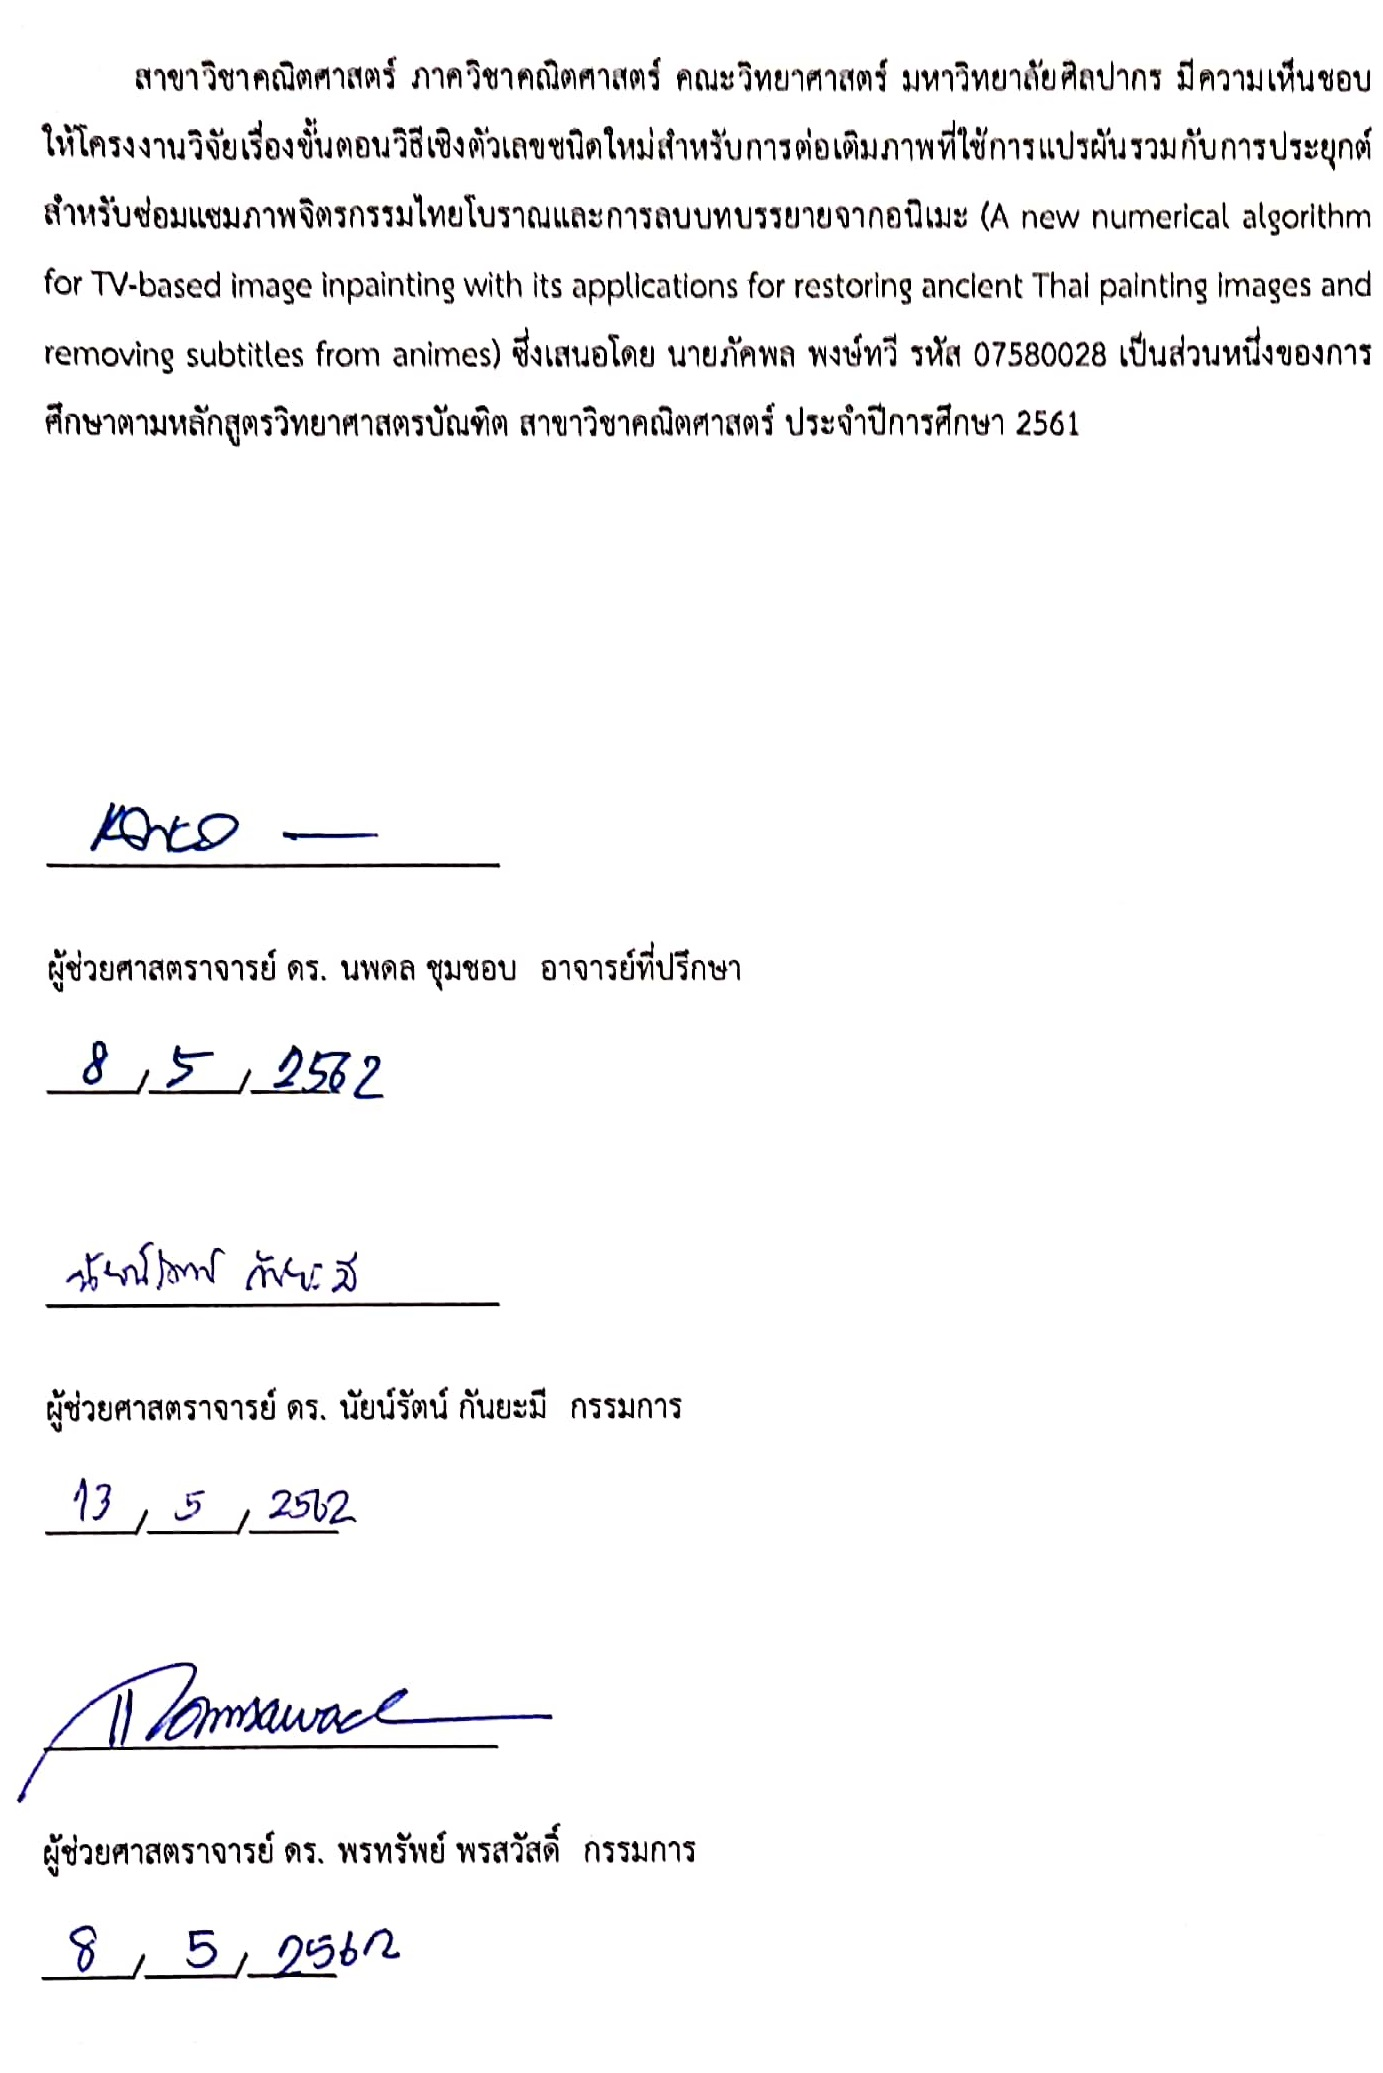
\includegraphics[width=\linewidth]{image/approval_letter/approval.jpg}
\end{figure}
\clearpage

%\backcover{\hspace{1cm}สาขาวิชาคณิตศาสตร์ ภาควิชาคณิตศาสตร์ คณะวิทยาศาสตร์ มหาวิทยาลัยศิลปากร มีความเห็นชอบให้โครงงานวิจัยเรื่องขั้นตอนวิธีเชิงตัวเลขชนิดใหม่สำหรับการต่อเติมภาพที่ใช้การแปรผันรวมกับการประยุกต์สำหรับซ่อมแซมภาพจิตรกรรมไทยโบราณและการลบบทบรรยายจากอนิเมะ (A new numerical algorithm for TV-based image inpainting with its applications for restoring ancient Thai painting images and removing subtitles from animes) 
%ซึ่งเสนอโดย นายภัคพล พงษ์ทวี รหัส 07580028 เป็นส่วนหนึ่งของการศึกษาตามหลักสูตรวิทยาศาสตรบัณฑิต สาขาวิชาคณิตศาสตร์ ประจำปีการศึกษา 2561}
%{ผู้ช่วยศาสตราจารย์ ดร. นพดล  ชุมชอบ}
%{ผู้ช่วยศาสตราจารย์ ดร. นัยน์รัตน์ กันยะมี}
%{ผู้ช่วยศาสตราจารย์ ดร. พรทรัพย์  พรสวัสดิ์}

%\newpage